\section{Related work and motivation}\label{sec:2:motivation}
Within the field of process mining, research on and use of predictive modelling techniques has attracted plenty of attention in the last five years. PPM techniques are usually developed with a specific purpose in mind, ranging from next activity prediction~\cite{evermann2017predicting,DBLP:conf/caise/TaxVRD17}, over remaining time prediction~\cite{verenich2019survey}, to outcome prediction~\cite{kratsch2020machine}. For a systematic literature review of the field, we refer to~\cite{neu2021systematic}. 
Beyond the PPM field, this work is related to previous research on stage-based process mining~\cite{nguyen2016business}, in which a technique is presented to decompose an event log into stages, and work on the detection of time granularity in event logs ~\cite{pourbafrani2020}. 
%Nonetheless, in this work, we employ a more straightforward aggregation, either equitemporal or equisized (cfr. Section~\ref{sec:3a:preliminaries}). 
%\todo[inline]{I find the "nonetheless" sentence confusing. I apparently connects to a point the Pourbafrani paper that is not discussed. And I think also this detailed point should not be discussed here. So the "nonetheless" sentences should be dropped imho. \\Also, I do not understand why Pourbafrani is the only author singled out to be named. Is this paper so striking important? Imho not. So just speak of the paper, not of the author like for all the other papers.}

The shift from fine-granular PPM techniques, including next activity, remaining time, and outcome prediction, to model-based prediction, allows to obtain new insights into the global development of the process.
Consider the example in Figure~\ref{fig:dfg_example_intro} where the road fine traffic management event log\footnote{\url{https://doi.org/10.4121/uuid:270fd440-1057-4fb9-89a9-b699b47990f5}} is partitioned into 100 intervals in which an equal number of DF relations occur.
\begin{figure}
    \centering
    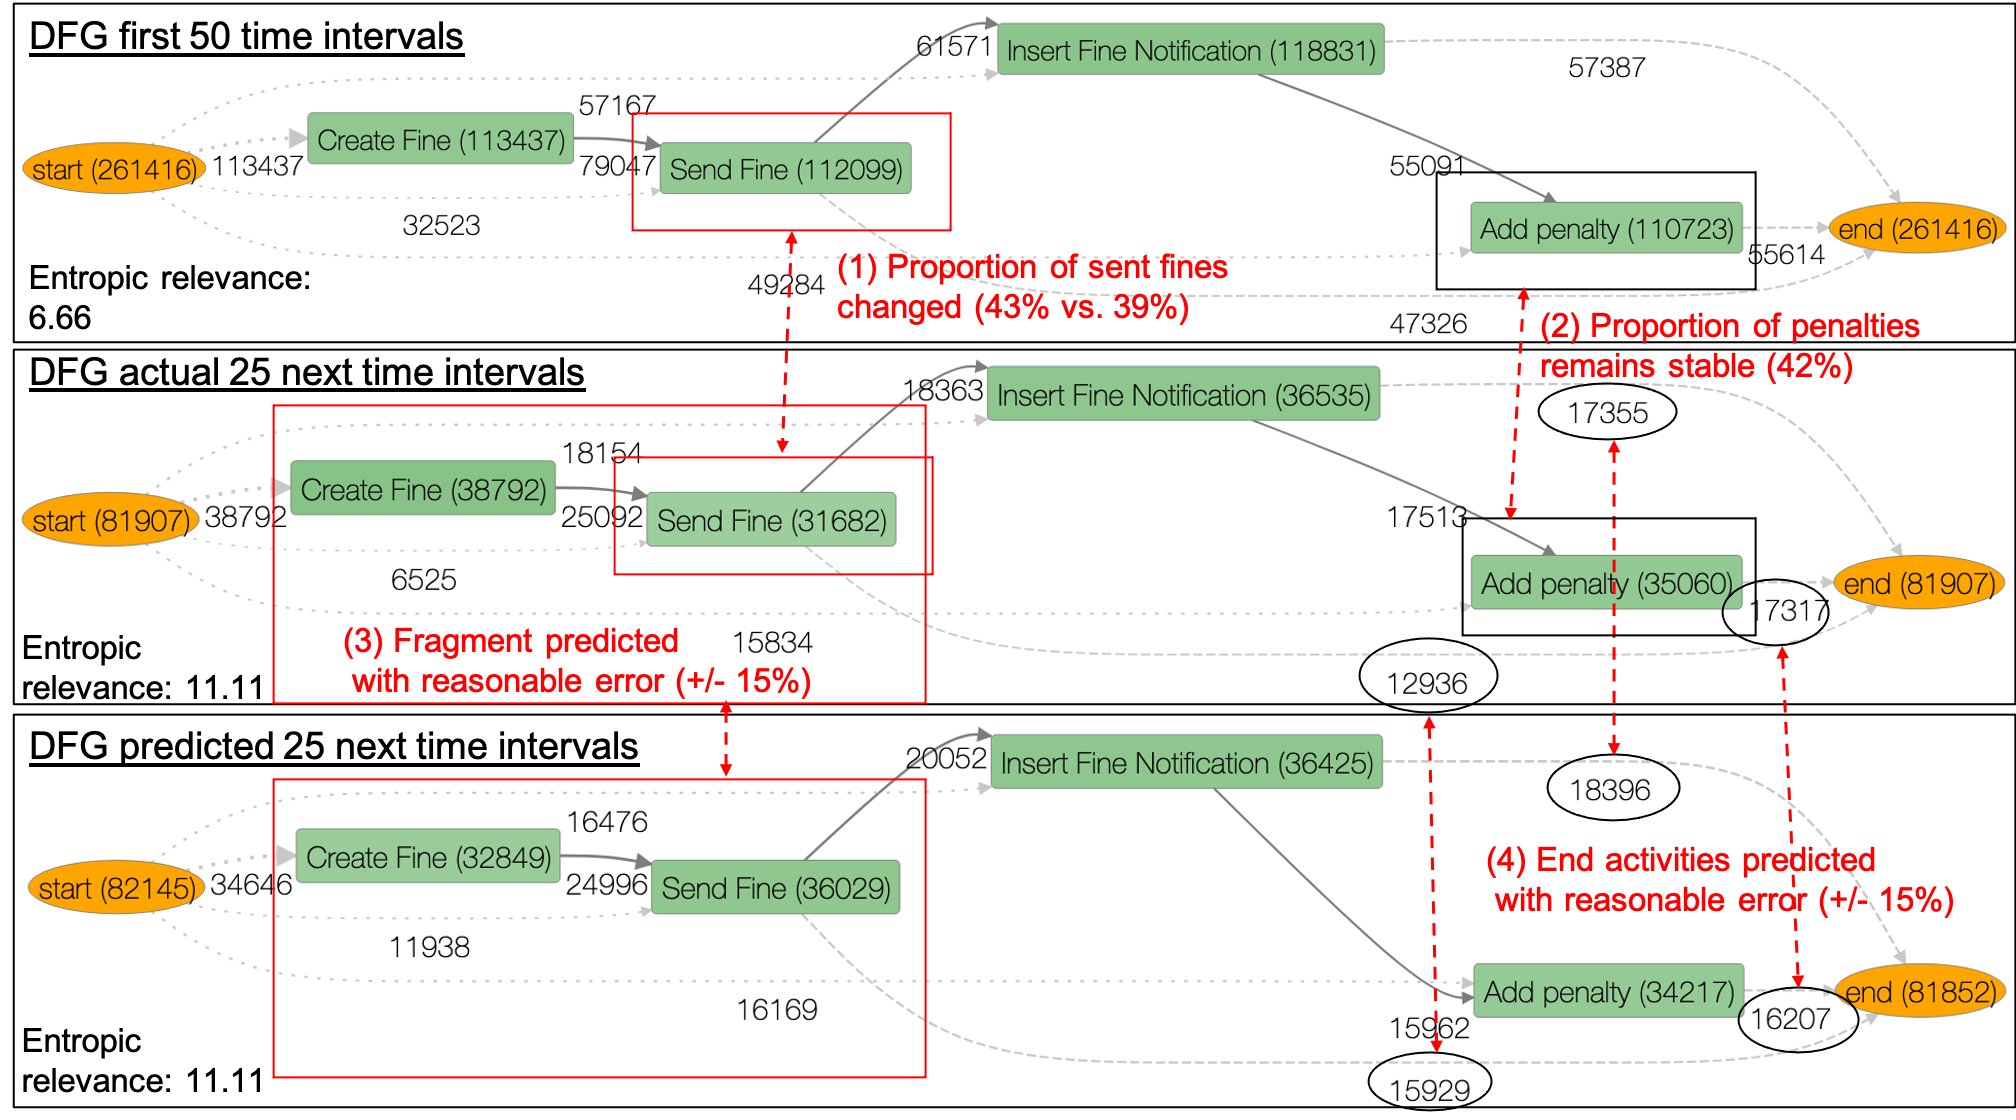
\includegraphics[width=\textwidth]{img/MotExample.png}
    \caption{Directly-follows graphs of the 50 first intervals of the event log, as well as a forecasted and actual DFG of the 25 next intervals.}
    \label{fig:dfg_example_intro}
\end{figure}
The DFs in the first 50 intervals are used to predict the next 25 intervals.
The DFGs show how process model forecasting and change exploration can provide multiple unique insights at a glance:
\begin{enumerate}
    \item Compared to the initial 50 intervals the proportion of fines sent decreases in the later intervals;
    \item The proportion of penalties added remains comparable between the first 50 and next 25 time intervals;
    \item The number of occurrences and arc weights between \emph{Create Fine} and \emph{Send Fine} are predicted with reasonable error (+\-15\%);
    \item The arc weights of the ending activities are predicted with reasonable error (+\-15\%).
\end{enumerate}
These provide insight both in terms of the past and present model ((1)-(2)) and the quality of forecasts between the actual and forecasted model ((3)-(4)).
Being able to construct such forecasts allows stakeholders to make estimates regarding how the overall fine system will evolve and allows to answer questions such as ``How many more fines will be received?'', ``Will the backlog of fines be reduced?'', ``Will all fines be paid'', and `Will the ratio of unpaid fines stay the same?'
This motivating example shows that, where process mining focuses on learning the as-is model to reason about trajectories of future cases and suggest potential repairs and improvements, process model forecasting allows to grasp the future stage of the overall process model in terms of a will-be model. % outcomes of the current as-is process, which allows to shortcut potentially wrong outcomes. 
%\todo[inline]{I found this shortcut-wrong statement hand wavy and misleading. I deleted it.}

A suitable means to evaluate the forecasts quantitatively is entropic relevance \cite{DBLP:conf/icpm/PolyvyanyyMG20}. This measure captures the quality of the discovered and forecasted DFGs with respect to the event logs they represent. 
Entropic relevance penalises the discrepancies in the relative frequencies of traces recorded in the log and described by the DFG as it stands for the average number of bits used to encode a log trace using the DFG, with small values being preferable to large ones.
If the entropic relevance of the forecasted DFG and the actual future DFG with respect to the test log is the same, it suggests that both DFGs represent the future behaviour similarly well. 
The entropic relevance of the historical DFG derived from the training log with respect to the testing log is 6.66 as indicated in Figure \ref{fig:dfg_example_intro}, 
%\todo[inline]{you refer to Fig 1 here, right? Please make that explicit.}
suggesting that the future behaviour shifts and the historical DFG still represents the behaviour in the log better than both the actual and forecasted DFGs which sit at an entropic relevance of 11.11. 

Measurement values are not enough to fully reveal the change of behaviour to the analyst. To this end, we complement the model-level prediction technique with a visualisation system to enable analysts to understand the forthcoming changes to the processes. Various process analysis tasks benefit from process forecasting~\cite{DBLP:conf/bpm/PollPRRR18}, most notably process forecasting helps understanding the incremental changes and adaptations that happen to the process model and to project them into the future. In terms of visualisation principles, we follow the ``Visual Information-Seeking Mantra":~\emph{overview first, zoom and filter, then details-on-demand}~\cite{DBLP:conf/vl/Shneiderman96}. 
%(maybe talk about tasks? not requirements)
Thus, we expect the design of our visualisation system to assist in the following tasks:

\begin{requidescr}
	\item[Identify process adaptations:\namedlabel{req:adaptation}] The visualisation system should assist the user in identifying the changes that happen in the process model of the future in respect to the past;
	\item[Allow for interactive exploration:\namedlabel{req:interactive}] The user should be able to follow the visual information-seeking principles, including overview first, filtering, zooming, and details-on-demand.
\end{requidescr} % CUSTOM from CDC, with love :)

Forecasting entire process models provides a new perspective on predictive process monitoring. 
%Observe that our process model forecasting technique intrinsically puts forwards an entirely new perspective on predictive process monitoring. 
The prediction horizon is substantially longer as compared to what existing next-activity prediction models can achieve. Moreover, where next activity and related PPM techniques have a strong case-level focus, a prediction at the model level provides a more comprehensive picture of the future development of the process.

%\todo[inline]{What comes now as "please..." is unspecific speculation. I tried to eliminate references to our technique in Section 2 altogether. Our technique must be in Section 3. Section 2 is for requirements and other works. However, "please..." goes even further beyond what we actually do. So best simply delete it. It just confuses the reader.}
%Please note that process model forecasting could partially assume goal-oriented prediction, as the forecast DFG allows to answer multiple oftentimes used goal statements pertaining to the execution of a particular activity, or a precedence relationship of a particular activity pair \cite{DBLP:journals/tkdd/TeinemaaDRM19} at the same time. However, our technique is not intended to ``replace'' existing techniques, but rather posits a new yet complementary perspective on PPM.

%Note that the horizon is longer compared with next-step prediction, and that these results would only be obtainable if long next-step predictions were performed.
%Hence, both are complementary by their being used as varying horizons to obtain a full picture of the future development of a process (model).
%Process model forecasting remains complementary with remaining time prediction as well, which could indicate what activities lead to what remaining time.
%The process model forecast can partially assume goal-oriented prediction, as the forecast DFG allows to answer multiple oftentimes used goal statements pertaining to the execution of a particular activity, or a precedence relationship of a particular activity pair \cite{DBLP:journals/tkdd/TeinemaaDRM19} at the same time.
